\documentclass[conference]{IEEEtran}
\IEEEoverridecommandlockouts
% The preceding line is only needed to identify funding in the first footnote. If that is unneeded, please comment it out.
\usepackage{cite}
\usepackage{amsmath,amssymb,amsfonts}
\usepackage{algorithmic}
\usepackage{graphicx}
\usepackage{textcomp}
\usepackage{xcolor}
\usepackage{subfig}


\def\BibTeX{{\rm B\kern-.05em{\sc i\kern-.025em b}\kern-.08em
    T\kern-.1667em\lower.7ex\hbox{E}\kern-.125emX}}
\begin{document}

\title{Clustering-based Ranking of Universities\\}

\author{\IEEEauthorblockN{George Matlis}
\IEEEauthorblockA{\textit{Department of Informatics} \\
\textit{University of Western Macedonia}\\
Kastoria, Greece \\
giorgos\_matlis@hotmail.com}
\and
\IEEEauthorblockN{Nikolaos Dimokas}
\IEEEauthorblockA{\textit{Department of Informatics} \\
\textit{University of Western Macedonia}\\
Kastoria, Greece \\
ndimokas@uowm.gr}
\and

\IEEEauthorblockN{Petros Karvelis}
\IEEEauthorblockA{\textit{Department of} \\
\textit{Informatics and Telecommunications} \\
\textit{University of Ioannina}\\
Arta, Greece \\
pkarvelis@uoi.gr}
}


\maketitle

\begin{abstract}
In recent year, there has been an increasing interest among international organizations and academic communities in the evaluation and ranking of educational institutions. Such rankings are of great significance to various stakeholders, including students and their families, academic staff, funding agencies, and universities themselves. Ranking methodologies typically involve the use of diverse indicator categories, aimed at ensuring objectivity and reflecting the relative importance of each university. These categories may include, but are not limited to, research output and impact, teaching quality and learning environment, international diversity, and reputation in the employment market. Apart from conventional ranking methods, clustering-based techniques can also be used to group universities according to their common characteristics and to evaluate their performance within each cluster. In this study, we seek to explore how universities from various regions can be clustered into distinct groups and ranked based on their unique features. For this purpose, we employ various clustering algorithms, each possessing distinct characteristics, and we present the similarities between them to obtain the most effective evaluation. We also analyze how university features can impact the evaluation and classification process into a cluster. We present some statistical results of university rankings and finally, we visualize the clustering process to facilitate a deeper understanding of the findings.
\end{abstract}

\begin{IEEEkeywords}
University Rankings, Clustering, Quacquarelli Symonds
\end{IEEEkeywords}

\section{Introduction}
The selection of an excellent university is pivotal in securing a high-quality education, offering students a robust foundation of knowledge, skills, and credentials. Furthermore, it may lead to enhanced job opportunities with higher remuneration post-graduation as employers are more inclined to hire graduates from prestigious universities. Additionally, for students interested in academic research, top institutions generally employ subject matter experts and possess well-funded research programs. Such institutions provide students with the opportunity to partake in pioneering research, acquire invaluable experience, and develop skill sets essential for their future endeavors. \\
In order to help people in the decision-making process of choosing a great university, many organizations like the Academic Ranking of World Universities (ARWU), Quacquarelli Symonds (QS), Times Higher Education World University Rankings (THE), provide ranking lists to evaluate universities. All these organizations base their ranking lists on several indicators such as the academic reputation of a university, the ratio of the number of students and faculty staff, the total number of academic citations, the number of international students and faculty staff, etc. Each indicator usually has a corresponding weight to signify its importance of evaluating a university. By examining the indicators used by the aforementioned organizations, we can briefly sum up a few things that were mentioned in \cite{b9}: \\

\begin{itemize}
    \item The similarity of indicators among ranking lists is low, which means that organizations use mostly different indicators to evaluate universities. 
    \item The weight that is used to signify the importance of an indicator, may be different among ranking lists. 
    \item The research production and impact related indicators among ranking lists are similar. \\
    
\end{itemize}

Besides of helping students make informed decisions for their future, university rankings can encourage and guide universities to perform better in areas like research, teaching, and internationalization that are crucial to their stakeholders. \\
Although they have significant benefits, university ranking methods come with a few drawbacks: \\

\begin{itemize}
    \item \textbf{Subjectivity} - Ranking systems frequently depend on data that is hard to compare or verify across different nations and cultures. Rankings may become skewed and inaccurate as a result of this. 
    \item \textbf{Overemphasis on Research} - Several university rankings give priority to research production and citations, which may encourage universities to place more focus on research than on other aspects of higher education such as teaching and community participation. 
    \item \textbf{Negative Effects on Higher Education} - Competition between institutions brought on by university rankings may have detrimental effects on higher education. For instance, institutions may prioritize raising their ranking over other objectives or may act unethically, such as by providing false data, in order to do so. 
    \item \textbf{Lack of Transparency} - Certain university ranking systems are not openly disclosed or transparent, which can make it challenging for stakeholders to comprehend how the rankings are determined and to judge the credibility and validity of those rankings. \\
\end{itemize}

Grouping universities according to specific traits or criteria, might help people make more educated decisions about where to study or work by giving a more detailed view of their strengths and shortcomings. A few reasons why grouping universities may be a more desirable process than to simply rank them from best to worst are: \\

\begin{itemize}
    \item \textbf{A limitation of criteria} - Ranking methods typically use a limited set of criteria to evaluate the performance of each university, but some universities are performing very well in different areas of expertise, so grouping them can highlight their strengths. 
    \item \textbf{Diverse needs} - Each individual has different priorities when choosing a university, such as, cost, location and academic courses. 
    \item \textbf{Avoiding Stigma} - By ranking universities from best to worst, a hierarchy can be created that stigmatizes lower-ranked schools and deters potential students from applying. This effect can be lessened and a more favorable and inclusive perspective of universities can be provided by grouping universities based on specific traits or areas of specialization. \\
\end{itemize}

This study aims to resolve some of the issues mentioned above by clustering and ranking universities with similar traits.

\section{Related Work}
Clustering is a machine learning technique that belongs to the category of unsupervised learning and aims to group related objects together into distinct clusters. \\
There are several different types of clustering, each with it's benefits and drawbacks. Some of the types of clustering are: \\


\begin{itemize}
    \item \textbf{Hierarchical} - With this technique, clusters are organized into a tree-like structure, with each smaller cluster being a subset of a bigger cluster. Agglomerative \cite{b1} and divisive hierarchical clustering \cite{b2} are the two forms. Each data point begins in its own cluster when using agglomerative clustering, and the process eventually merges all clusters into one. In divisive clustering, all data points begin in a single cluster and are subsequently split into smaller clusters by the algorithm. 
    \item \textbf{K-Means} - One of the most popular clustering techniques is known as K-means clustering \cite{b3}. The data must be divided into K clusters, where K is an adjustable parameter. The approach seeks to reduce the sum of the squared distances between each data point and the cluster center to which it has been assigned.  
    \item \textbf{Fuzzy Clustering} - This technique enables a data point to have varying degrees of membership in many clusters. Fuzzy C-Means (FCM) clustering \cite{b4} is the most widely used fuzzy clustering algorithm. 
    \item \textbf{Density-Based} - Data points that are close to one another in a high-density area and are separated by areas of lower density are grouped using the density-based clustering technique. DBSCAN \cite{b5} is the most popular density-based clustering algorithm (Density-Based Spatial Clustering of Applications with Noise). 
    \item \textbf{Model-Based} - This technique posits a blend of probability distributions as the source of the data points. Gaussian Mixture Models \cite{b6} are the most used model-based clustering approach (GMM). \\
\end{itemize}

Much research has been done regarding the performance ranking of universities, university departments, and general academic related branches. \\  
A famous technique for ranking universities is the rank fusion \cite{b11}. Rank fusion, also known as meta-ranking, is a technique for combining the results of multiple university rankings to create a more comprehensive and reliable ranking. Rank fusion works by standardizing the different rankings and combining the results using a weighted average, where the weights reflect the importance of each ranking. 
Compared to separate ranking algorithms or sources, rank fusion can offer a number of advantages. It can give a more steady and reliable rating and lessen the influence of outliers or inaccuracies in individual rankings. Also, it may take into account a broader range of factors or viewpoints and offer a more complete picture of the effectiveness or caliber of the ranking entities. Rank fusion should be used with caution, as the weights used to combine the rankings may be subjective or biased. \\
The rainbow ranking \cite{b10} is a famous ranking algorithm, that offers individual rankings for several facets of a university's success, including research, teaching, internationalization, and community participation, in contrast to typical university rankings that only offer a single overall score. Although rank fusion and rainbow ranking are related concepts, rainbow ranking is a specific method of rank fusion. For each factor, each university is given a ranking independently, and the results are added together to provide an overall rainbow ranking. The rainbow rating aims to give universities a more thorough and nuanced assessment of their performance and to assist them in identifying areas for improvement. The rainbow ranking's recognition of the diversity of universities and the many objectives and priorities they may have is one of its main benefits. For instance, a university that places a high priority on teaching might rank well in that category even if it falls short in other categories. As an alternative to conventional university rankings, the rainbow rating has been adopted by various organizations and universities, and it has received recognition for its inclusivity and thoroughness. It has, however, also drawn criticism for being overly complicated and making it impossible to compare universities across multiple categories. \\
%Regarding the clustering of the aforementioned, due to the complexity of the process and the difficulty of drawing conclusions, the amount of research that has been conducted is limited. \\
For our study, we relied on \cite{b7}, although \cite{b8} is pretty similar to our analysis. In \cite{b7}, the researchers clustered universities from the National Taiwan University(NTU) ranking using the DBSCAN, EM \cite{b15} and K-Means algorithms, ending up to the conclusion that K-Means is the most appropriate one because its results are the closest to the NTU ranking. The clustering results they obtained through experimentation with 12 and 43 clusters resembles the rankings of the NTU.  
In \cite{b8}, the Quacquarelli Symonds (QS) dataset for the year 2022 was used for clustering and analysis. The researcher used 6 score indicators which we mention in section 3 and chose the Gaussian Mixture Model (GMM) as the main algorithm for clustering. The optimal number of clusters was chosen to be 4 using the Akaike's Information Criteria (AIC) \cite{b12} and Bayesian Information Criteria (BIC) \cite{b13}. In contrast to the ranking system currently used by QS, the results revealed a new classification system for universities. \\
Comparing our work to \cite{b7} and \cite{b8}, we used the K-Means, GMM, Agglomerative and Fuzzy C-Means algorithms in order to provide a more diverse and nuanced perspective on the data, and to uncover different patterns and structures that may not be revealed by a single algorithm. Also, in addition to the 6 indicators that were used in \cite{b8}, we used 3 more indicators from the dataset that were meant to categorize universities, so as to have a more equal and fair classification of the universities. 
Finally, we used two techniques for normalizing the data that are mentioned in section 3.
%Finally, apart from normalizing the data the usual way, we multiplied each indicator by custom weight based on the importance of the indicator.


\section{Dataset and Data Pre-Processing}
\subsection{Dataset}
For the purposes of this study, we acquired a dataset from the official website of the Quacquarelli Symonds (QS) for the year 2023. In the dataset, there are over 1400 universities from all over the world including universities from diverse locations of Europe, Asia and North America. We chose the specific dataset because of the different indicators that are used to evaluate the performance of a university, unlike other university rankings that use only bibliographic related indicators. \\
Totally, there are 27 columns in the dataset but according to the QS ranking, each university is ranked and assessed using only 6 columns/indicators named: \\

\begin{enumerate}
    \item \textbf{Academic Reputation} (ar score) - Evaluates the teaching and research quality of the university.
    \item \textbf{Employer Reputation}( er score) - Evaluates how competent, innovative, and effective students and graduates are for the employment market.
    \item \textbf{Faculty/student ratio} (fsr score) - Evaluates how universities provide students with meaningful access to faculty staff.
    \item \textbf{Citations per faculty} (cpf score) - Evaluates the total number of academic citations in papers produced by a university in five years.
    \item \textbf{International student ratio \& International faculty ratio}(isr score \& ifr score) - Evaluates the ability of a university to attract foreign students and faculty staff from all over the world. \\
\end{enumerate}

The above mentioned indicators, each in turn get a percentage of \(40\%, 10\%, 20\%, 20\%, 5\%, \text{ and } 5\%\) of the total score. \\
In our analysis we include, in addition to the above, three more indicators named: \\

\begin{enumerate}
    \item \textbf{Size} - The total number of full time degree-seeking students.
    \item \textbf{Focus} - The broad subject areas of each university, e.g Arts, Humanities, Engineering and Technology, Natural Sciences etc.	
    \item \textbf{Age Band} - The age of each university. \\
\end{enumerate}

The three additional indicators have been chosen specifically because we can group universities based on their values, and rank them distinctly and equally. To elaborate further, for some cases, it would seem unfair to rank two universities on the same cluster that have distant values on the above indicators. An old university which has a large campus area can't be usually compared to a new university which has a small campus area. \\
Each of the three indicators captures a percentage of the total number of universities. \\

\begin{table}[ht]
    \begin{center}
        \caption{Size, Focus, Age Band}
        \renewcommand{\arraystretch}{1.25}
        \begin{tabular}{ |c|c|p{3.2cm}|c| } 
            \hline
            & Size & Students & Perc. (\%) \\
            \hline
            XL & Extra Large & More than \(30.000\) & 23.8 \\
            L & Large        & \(\geq 12.000\)  & 46.6  \\ 
            M & Medium       & \(\geq 5.000\)  & 23.8  \\ 
            S & Small        & Fewer than \(5.000\)  & 5.8 \\
            \hline
            & Focus & Faculty Area & \\
            \hline
            FC & Full comprehensive & 5 faculty areas \& medical school & 41.6 \\ 
            CO & Comprehensive      & 5 faculty areas & 32.5\\ 
            FO & Focused            & 3 or 4 faculty areas & 22.0 \\ 
            SP & Specialist         & 2 or fewer faculty areas & 3.9 \\
            \hline
            & Classification & Age & \\
            \hline
            5 &	Historic    &	100 years old and more & 37.5\\
            4 &	Mature      &	50-99 years old & 34.4\\
            3 &	Established & 	25-49 years old & 20.4\\
            2 &	Young       &	10-24 years old & 6.7\\
            1 &	New         &	Less than 10 years old & 0.9\\
            \hline
        \end{tabular}
    \end{center}
\end{table}

\subsection{Data Pre-Processing}

After describing the indicators that were used for our analysis, some pre-processing of the data is a desirable prerequisite to clustering. First and foremost, we have to exclude the universities that have missing values on at least one of the above 9 indicators, with the purpose of evaluating them equally. We convert the size and the focus indicators to a numerical value ranging from \(0 - 100\), so as to examine how each indicator affects all the other indicators. Thus, we calculate a correlation matrix using the Pearson correlation coefficient \cite{b6}. The resulting correlation matrix for the 9 indicators is


\begin{table}[ht]
    \begin{center}
        \caption{Correlation Matrix}
        \renewcommand{\arraystretch}{1.5}
        \begin{tabular}{|p{0.5cm}|c|c|c|c|c|c|p{0.4cm}|p{0.4cm}|p{0.2cm}|} 
            \hline
            & size & focus & age & ar & er & fsr & cpf &   ifr & isr \\
            \hline
            size        & 1 &  &  &  &  &  &  &  &  \\
            \hline
            focus       & 0.45 & 1 &  &  &  &  &  &  & \\
            \hline
            age    & 0.24 & 0.22 & 1 &  &  &  &  &  & \\
            \hline
            ar    & 0.32 & 0.37 & 0.3 & 1 &  &  &  &  & \\
            \hline
            er    & 0.19 & 0.23 & 0.21 & 0.84 & 1 &  &  &  & \\
            \hline
            fsr   & -0.2 & 0.09 & 0.12 & 0.38 & 0.35 & 1 &  &  & \\
            \hline
            cpf   & 0.1 & 0.21 & 0.16 & 0.57 & 0.44 & 0.12 & 1 &  & \\
            \hline
            ifr   & -0.08 & 0.11 & -0.03 & 0.4 & 0.35 & 0.17 & 0.45 & 1 & \\
            \hline
            isr   & -0.1 & 0.04 & 0.04 & 0.39 & 0.36 & 0.23 & 0.37 & 0.71 & 1 \\
            \hline
        \end{tabular}
    \end{center}
\end{table}

Examining the above table we can draw a few conclusions. The academic and employer reputation indicators have a relatively strong relation with most of the indicators and especially with one another. That implies that, as the academic reputation of a university increases, employers are more likely to hire students that graduated from that university. Also, there are some interesting things to note about the size, focus and the age band indicators. It seems that the 3 indicators do not have a strong relation with the other 6 indicators which means that, as the size, age, and the number of subject areas of a university increase, the other indicators do not get affected as much as we would except. An exception can be made about the academic reputation, which has the highest relation with the 3 indicators, but overall, size, age and broad subject areas do play a major role in the performance of a university. \\
Knowing which indicators are more important to our cluster analysis, we normalize the data. We used two techniques to normalize the data: \\

\begin{enumerate}
    \item We multiplied each indicator by a custom weight that is chosen based on the importance of the indicator. Then, we normalized their values to the scale 0 - 1. 
    \item We excluded all the weights from the normalization in order to have a more balanced and fair clustering. \\
\end{enumerate}

Each technique was used once per experimentation cycle. One experimentation cycle consists of clustering the data(using the algorithms at section 4) and calculating the similarity measure of the clustering algorithms. \\
The similarity measure is calculated using the rand index between every pair of algorithms. To compare the results of any algorithm with the QS ranking list we did the following: \\

\begin{enumerate}
    \item We created, for each experimentation cycle, \(N\) clusters \(N=7,24\). 
    \item In each cluster, we assigned \(\frac{\text{number of universities in QS rank list}}{N}\) universities. If there are remaining universities, we assign them in the last cluster. \\
\end{enumerate}

The normalization algorithm we used is the MinMaxScaler which can be described by the following equation \\

\begin{equation*}
    x_{\text{scaled}} = \frac{x - x_{\text{min}}}{x_{\text{max}} - x_{\text{min}}}
\end{equation*}


\section{Methodology}
\subsection{Clustering Algorithms}
For out cluster analysis, we used the following algorithms: \\

\begin{enumerate}
    \item \textbf{K-Means} - K-means can be a useful tool for university clustering in certain situations, particularly when simplicity, efficiency, and intuitive results are important. However, k-means would not perform well if the clusters are of different size and density and contain outliers.
    \item \textbf{GMM} - Assuming the data can be described as a combination of Gaussian distributions, GMM can be a valuable technique for university clustering. It can offer adaptability, interpretability, and outlier identification skills that can aid in improving comprehension and analysis of the performance of various university groups.
    \item \textbf{Agglomerative} - Agglomerative clustering can be used when a hierarchy of clusters is needed, or when flexibility and interpretability are important. However, it may not be the best choice for all situations, particularly when the underlying data has complex relationships or non-linear distributions.
    \item \textbf{Fuzzy C-Means} - Fuzzy C-Means is a useful algorithm for university clustering due to its ability to allow each university to belong to multiple clusters, with varying degrees of membership. Practically, for our case scenario, a university can be assigned to a specific cluster but it can also have a high probability of being a member of a neighbouring cluster. Thus, it helps us to make a more nuanced analysis of the performance and characteristics of different groups of universities. \\
\end{enumerate}

To find the optimal number of clusters using the 9 indicators we used: \\

\begin{enumerate}
    \item The EM algorithm with the default Weka values. EM assigns a probability distribution to each instance which indicates the probability of it belonging to each of the clusters. EM can decide how many clusters to create by cross validation.
    \item The Akaike Information Criterion (AIC) and the Bayesian Information Criterion (BIC) for a maximum of 30 clusters. The maximum number of clusters was chosen arbitrarily. Since AIC and BIC are both statistical measures used for model selection and comparison, we used the GMM algorithm for these measures.  \\
\end{enumerate}

The EM algorithm gave us 7 clusters. Using the AIC and BIC measures we came up with the graph that is shown in fig. 1. The number of clusters for the minimum value of BIC is 7 which is identical to the results of the EM algorithm. The number of clusters for the minimum value of AIC is approximately 29 but we used 24, as the difference between the AIC value of 29 and 24 clusters is quite small. \\


\begin{figure}[htbp]
\centerline{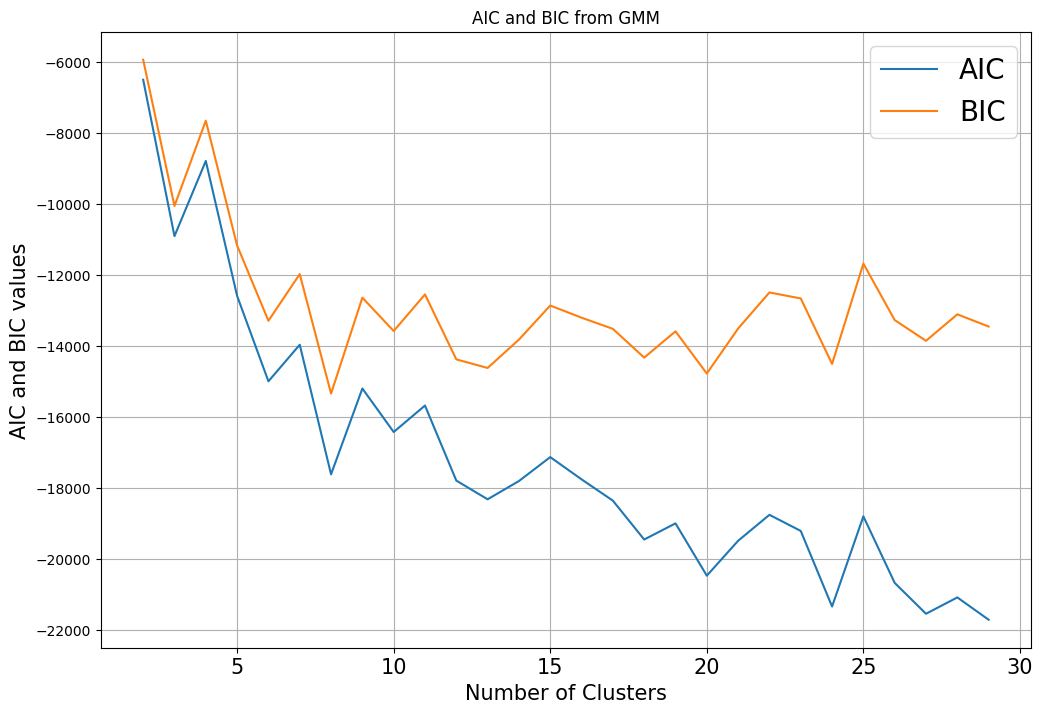
\includegraphics[scale=0.32]{AIC_BIC_NoWeights.png}}
\caption{AIC \& BIC values for a maximum of 30 clusters and a minimum of 2.}
\label{fig1}
\end{figure}

In order to visualize the clusters, we used the Multidimensional Scaling(MDS) algorithm \cite{b14} to reduce the initial dimensions of the data to 2. \\
The clustering results for 7 clusters and 9 indicators are shown in fig. 2. The sizes of each cluster for every algorithm are shown in table 3. The clusters are ordered based on the mean value of each cluster. The mean value of a cluster is calculated by adding the scores of each university in that cluster divided by 9. Then, adding the mean of each university divided by the size of the cluster we get the mean of the cluster. \\


\begin{figure}
    \centering

    \subfloat[a][K-Means]{
        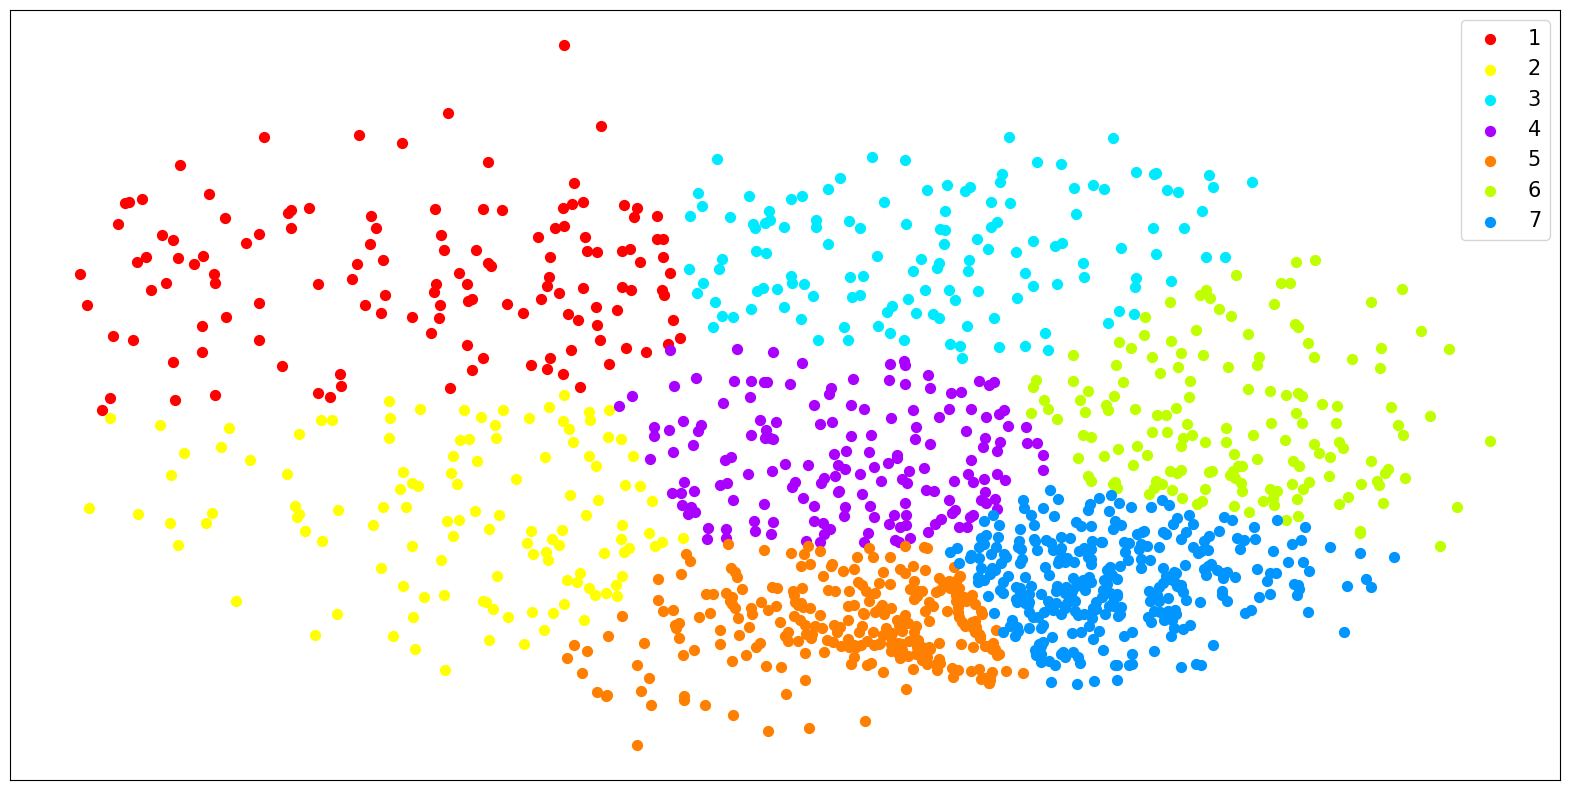
\includegraphics[scale=0.22]{kmeans_k7_noweights.png}
        \label{fig2}} \\

    \subfloat[b][GMM]{
        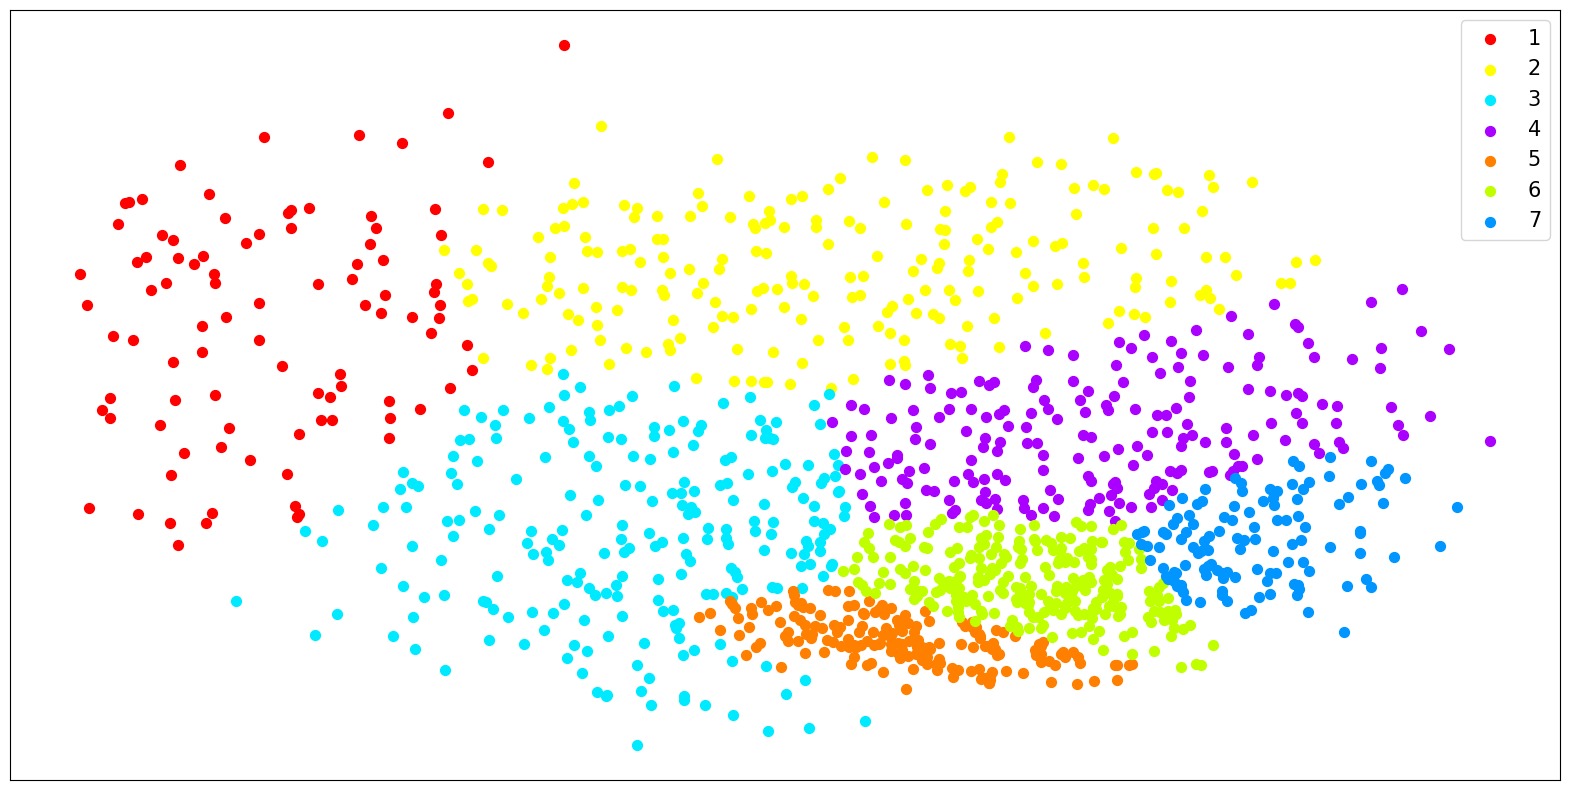
\includegraphics[scale=0.22]{gmm_k7_noweights.png}
        \label{fig3}} \\

    \subfloat[c][Agglomerative]{
        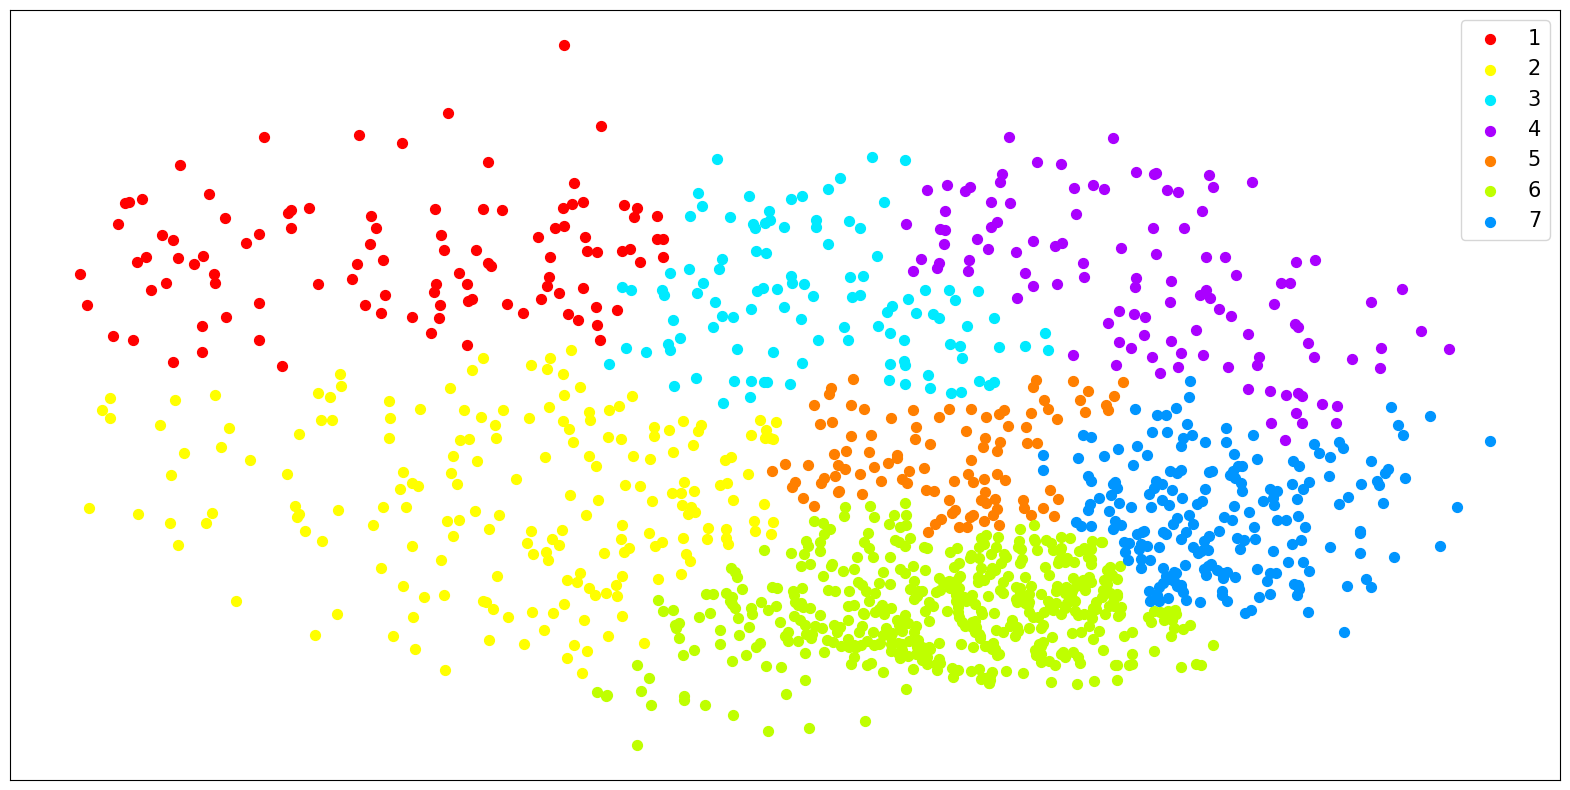
\includegraphics[scale=0.22]{agglomerative_k7_noweights.png}
        \label{fig4}} \\

    \subfloat[d][Fuzzy C-Means]{
        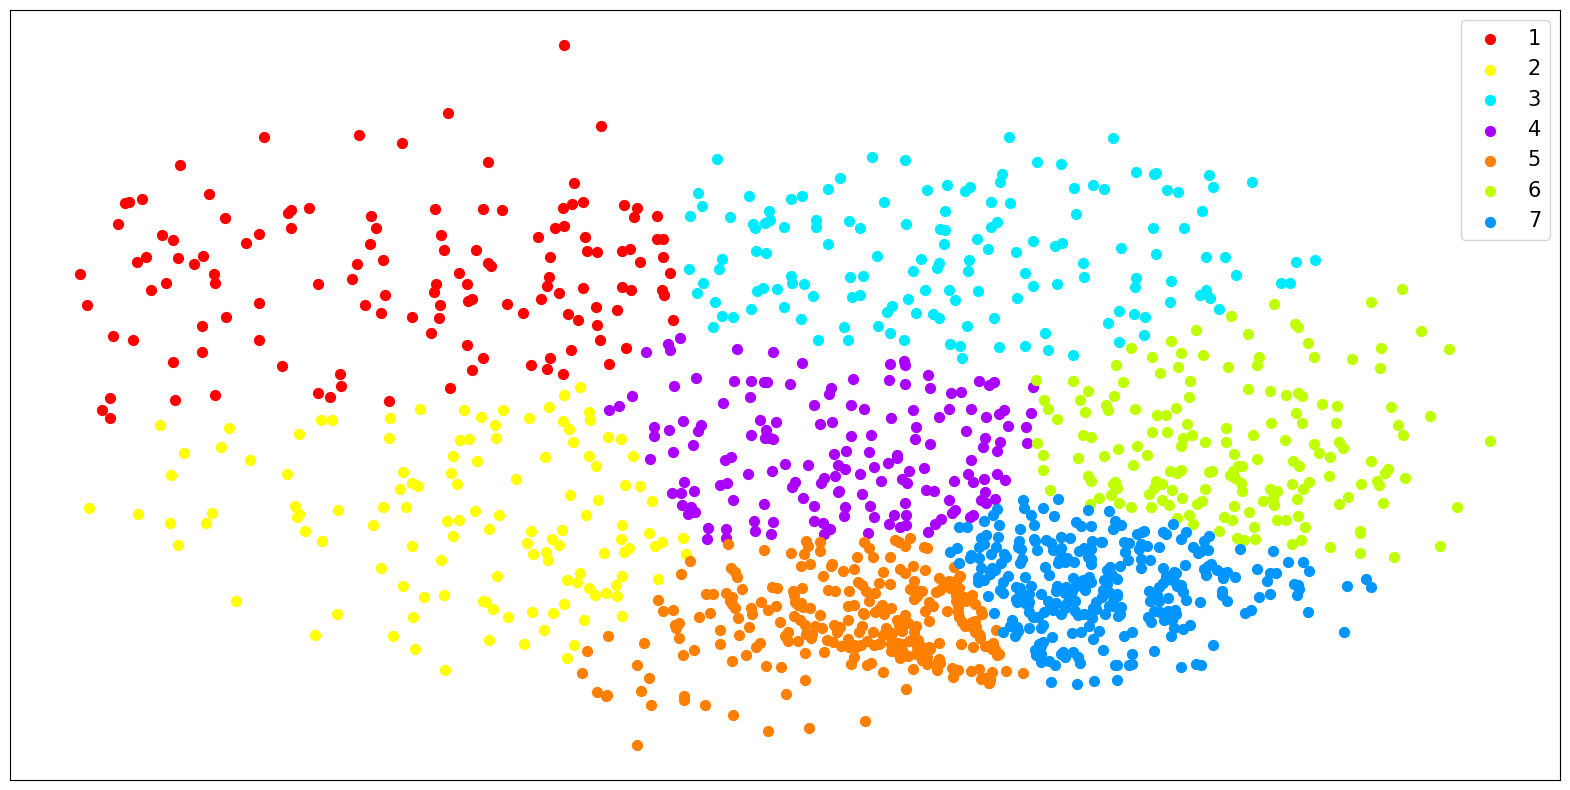
\includegraphics[scale=0.22]{fuzzycmeans_k7_noweights.png}
        \label{fig5}}

    \caption{K-Means, GMM, Agglomerative and Fuzzy C-Means for 7 clusters with 9 indicators.}
        
\end{figure}

%\begin{figure}[htbp]
%\centerline{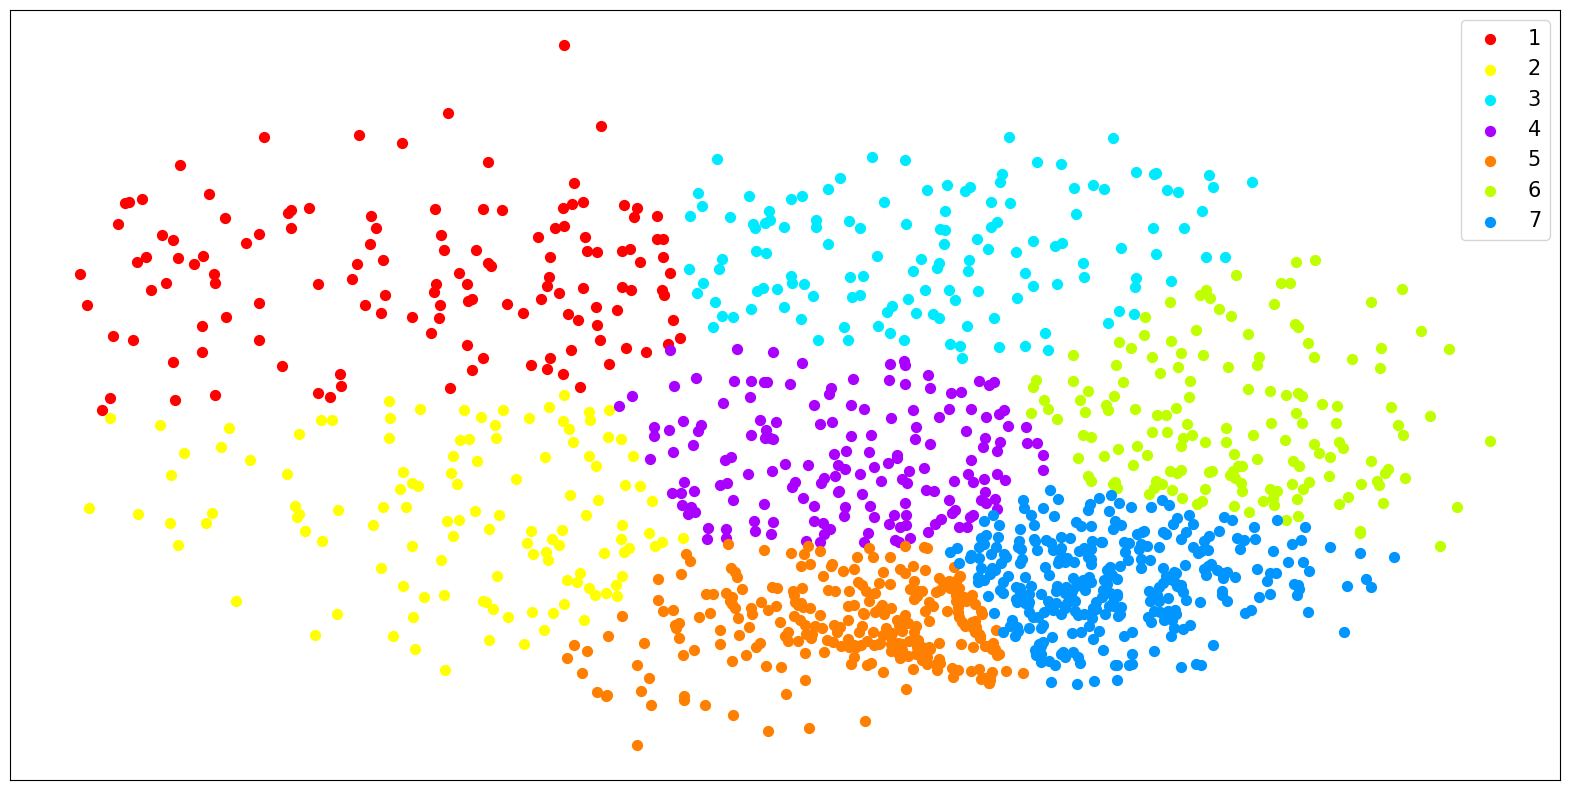
\includegraphics[scale=0.22]{kmeans_k7_noweights.png}}
%\caption{K-Means}
%\label{fig2}
%\end{figure}

%\begin{figure}[htbp]
%\centerline{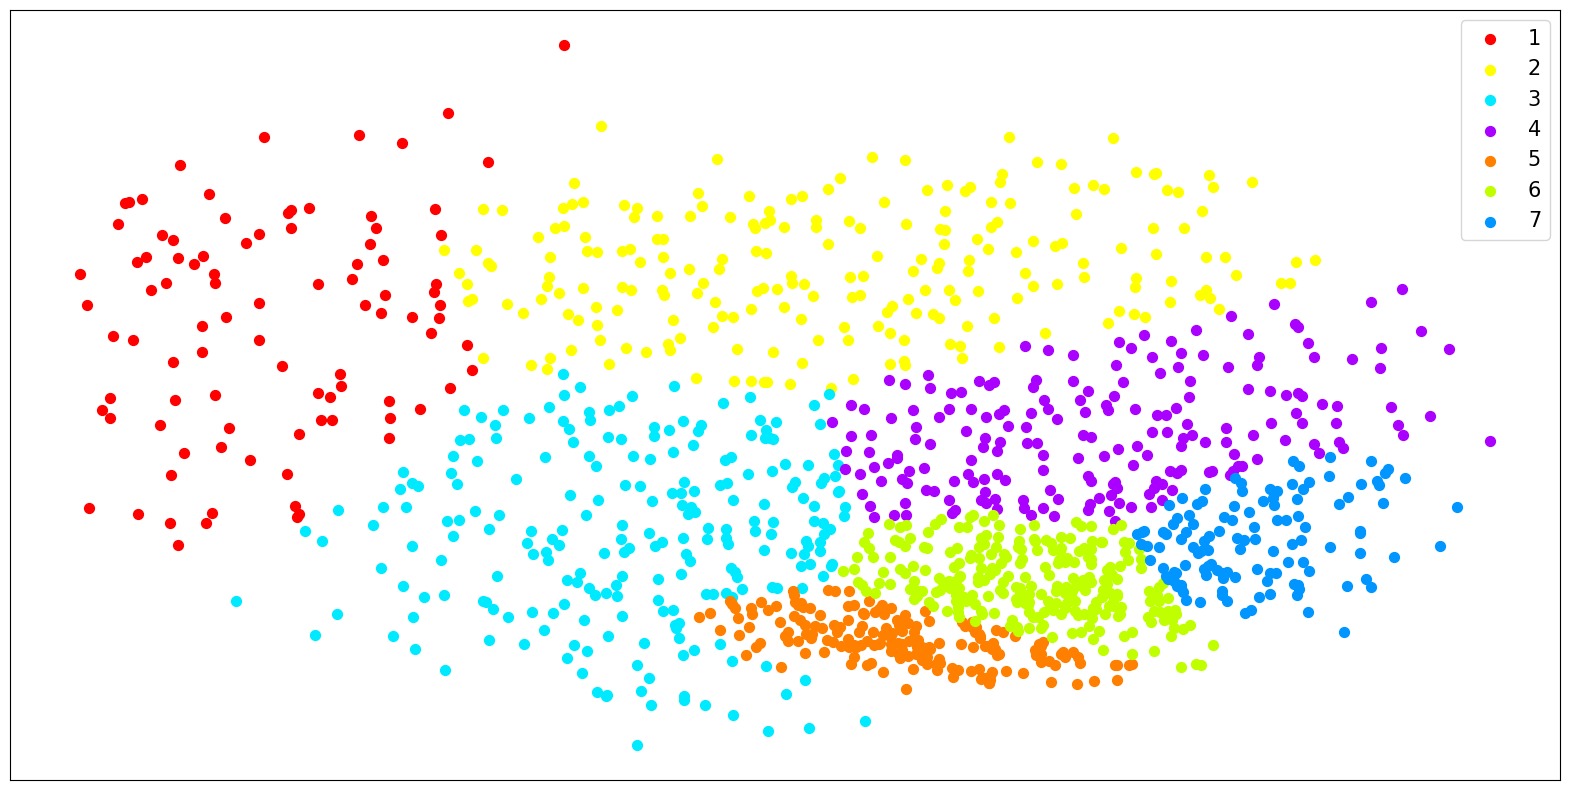
\includegraphics[scale=0.22]{gmm_k7_noweights.png}}
%\caption{GMM}
%\label{fig3}
%\end{figure}

%\begin{figure}[htbp]
%\centerline{\includegraphics[scale=0.22]%{agglomerative_k7_noweights.png}}
%\caption{Agglomerative}
%\label{fig4}
%\end{figure}

%\begin{figure}[htbp]
%\centerline{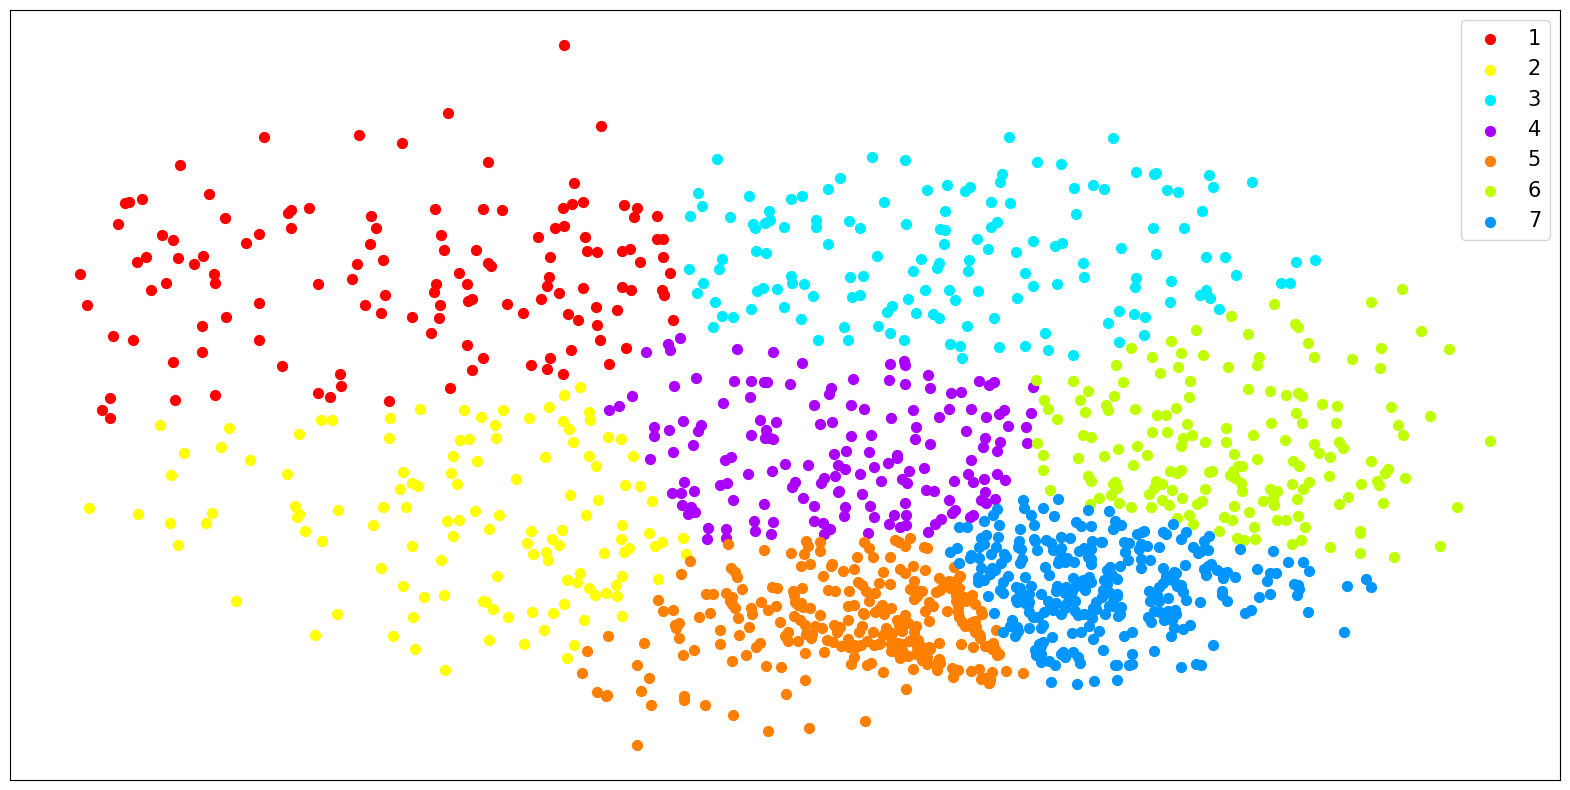
\includegraphics[scale=0.22]{fuzzycmeans_k7_noweights.png}}
%\caption{Fuzzy C-Means}
%\label{fig5}
%\end{figure}




\begin{table}[ht]
    \begin{center}
        \caption{Cluster Sizes for 7 clusters}
        \renewcommand{\arraystretch}{1.25}
        \begin{tabular}{ |c|c|c|c|c| } 
            \hline
            & KM & GMM & Agg & Fuzzy \\
            \hline
            1 & 133 & 94 & 105 & 131\\
            \hline
            2 & 124 & 222 & 194 & 127\\ 
            \hline
            3 & 137 & 233 & 111 & 151\\ 
            \hline
            4 & 171 & 200 & 114 & 165\\
            \hline
            5 & 271 & 182 & 106 & 272\\
            \hline
            6 & 158 & 255 & 470 & 171\\
            \hline
            7 & 314 & 122 & 208 & 291\\
            \hline
        \end{tabular}
    \end{center}
\end{table}



From visualizing the clustering algorithms and calculating the rand index(see table 4) we can make a few observations. First of all, the cluster with the highest mean(red cluster), for every algorithm, has a very low density and many outliers. That is to be expected because the size, focus and age band indicators of the universities that belong to that cluster, have mostly different values, whereas universities that belong to clusters with lower mean, have similar size, focus and age band indicator values. Thus, clusters with lower mean have higher density and fewer outliers. Regarding the shape of the clusters, K-Means and Fuzzy C-Means are pretty similar despite the fact that their rand score isn't very high. Although Fuzzy C-Means assigns a university to a cluster with a membership value, meaning that a university can belong to two different clusters with an equally high membership value, still, a university must be assigned to only one cluster. Examining the shape of clusters of K-Means and GMM an obvious difference can be observed. GMM can handle clusters with different shapes other than spherical. \\


\begin{table}[ht]
    \begin{center}
        \caption{Rand Index for 7 clusters}
        \renewcommand{\arraystretch}{1.25}
        \begin{tabular}{ |c|c|c|c|c|c| } 
            \hline
            & KM & GMM & Agg & Fuzzy & QS \\
            \hline
            KM & 1 &  &  &  &  \\
            \hline
            GMM & 0.726408 & 1 &  &  & \\ 
            \hline
            Agg & 0.854153 & 0.739578 & 1 &  & \\ 
            \hline
            Fuzzy & 0.813539 & 0.726609 & 0.819637 & 1 & \\
            \hline
            QS & 0.777024 & 0.753249 & 0.782652 & 0.78123 & 1 \\
            \hline
        \end{tabular}
    \end{center}
\end{table}

The clustering results for 24 clusters and 9 indicators are shown in fig. 3. We can see in table 5 that the rand score between every pair of algorithms has significantly increased. Also, using 24 clusters, the clustering results are now closer to the QS ranking. Considering that, we can conclude that as we increase the number of clusters, the similarity between every pair of algorithms and the initial QS ranking increases. \\

\begin{figure}
    \centering

    \subfloat[a][K-Means]{
        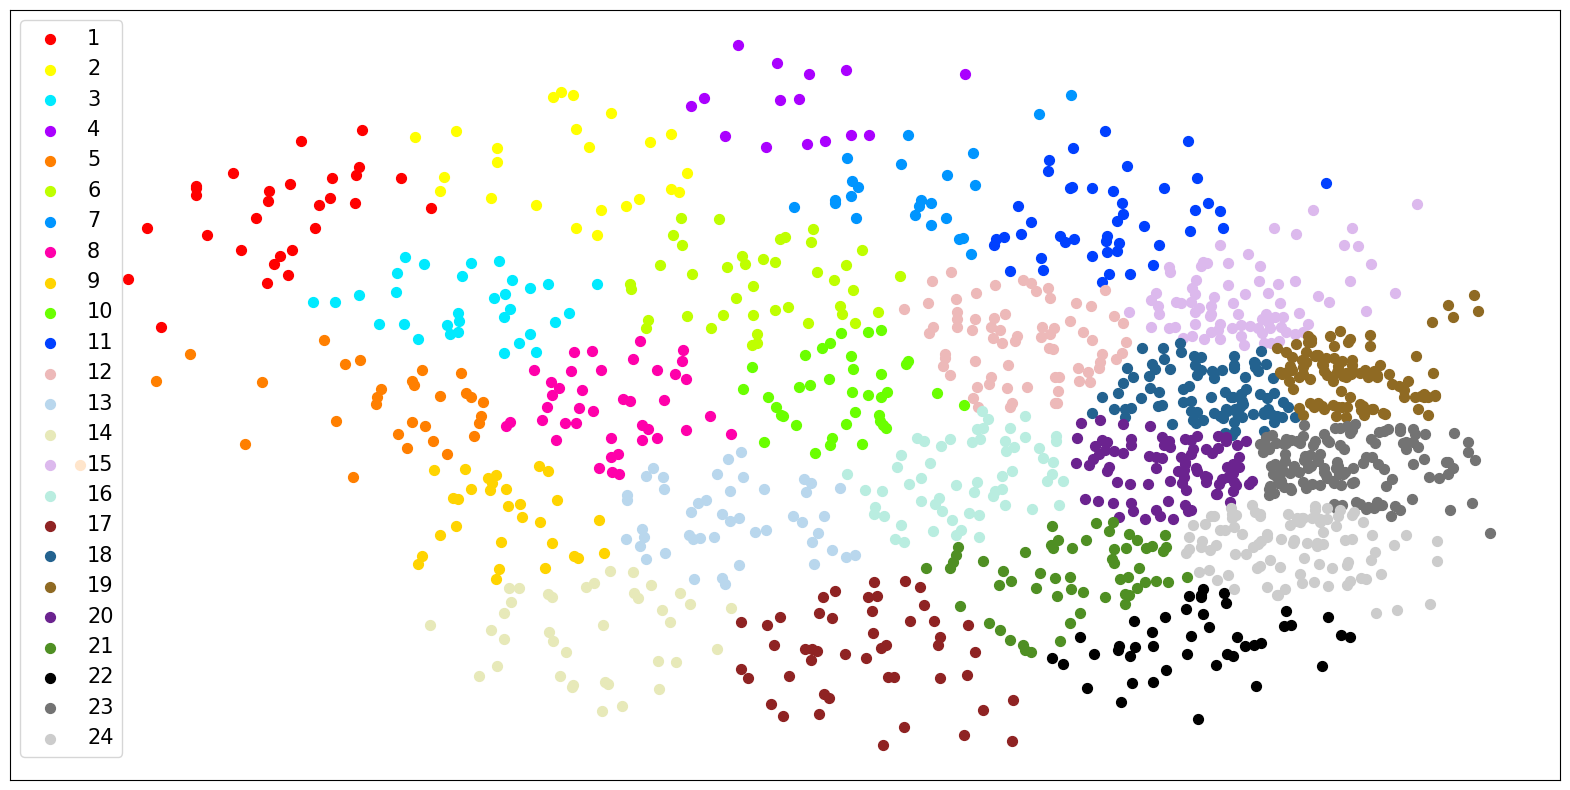
\includegraphics[scale=0.22]{kmeans_k24_noweights.png}
        \label{fig6}} \\

    \subfloat[b][GMM]{
        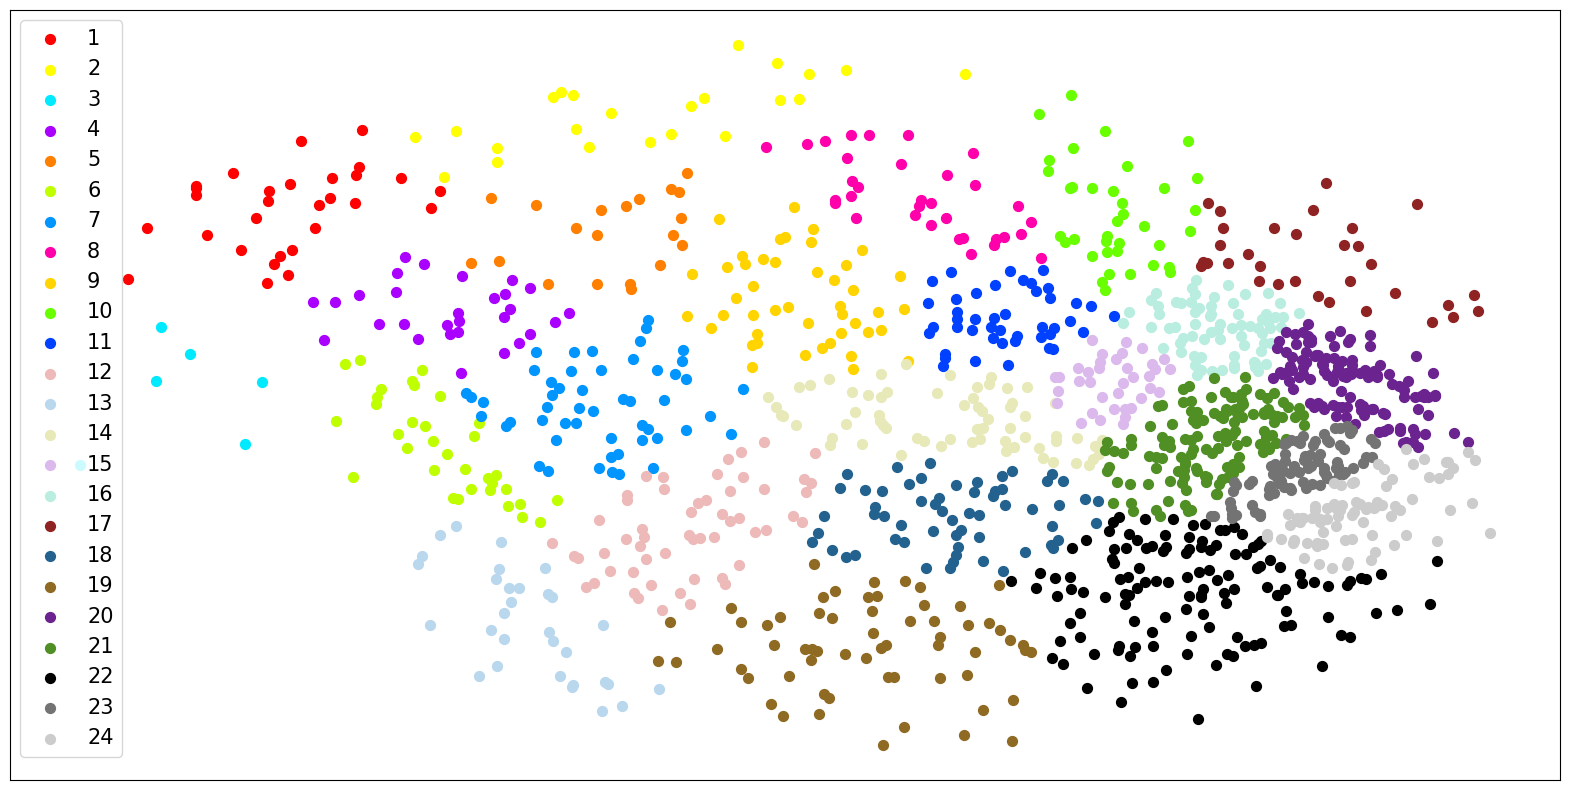
\includegraphics[scale=0.22]{gmm_k24_noweights.png}
        \label{fig7}} \\

    \subfloat[c][Agglomerative]{
        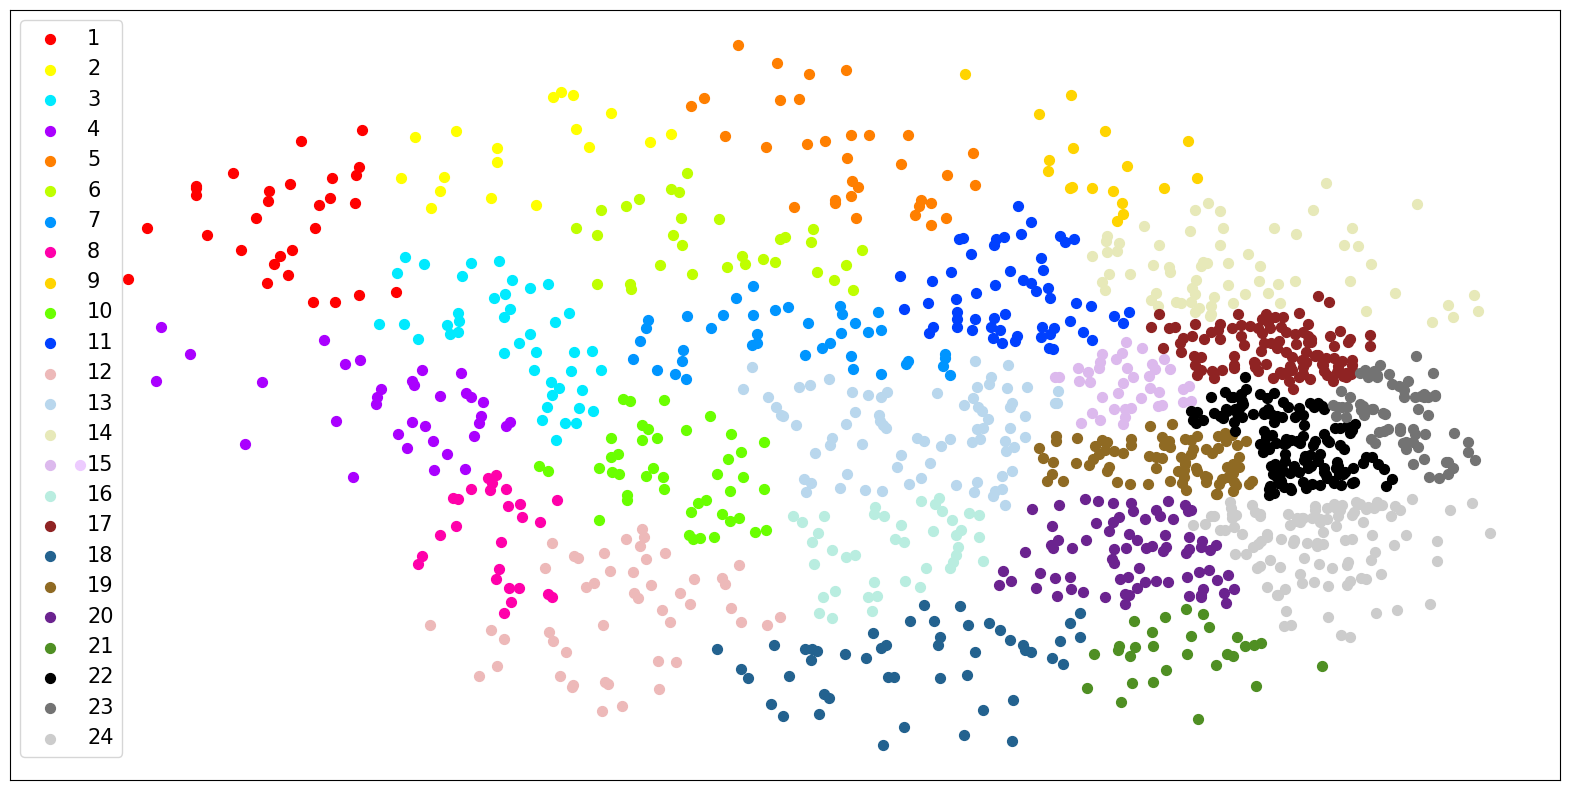
\includegraphics[scale=0.22]{agglomerative_k24_noweights.png}
        \label{fig8}} \\

    \subfloat[d][Fuzzy C-Means]{
        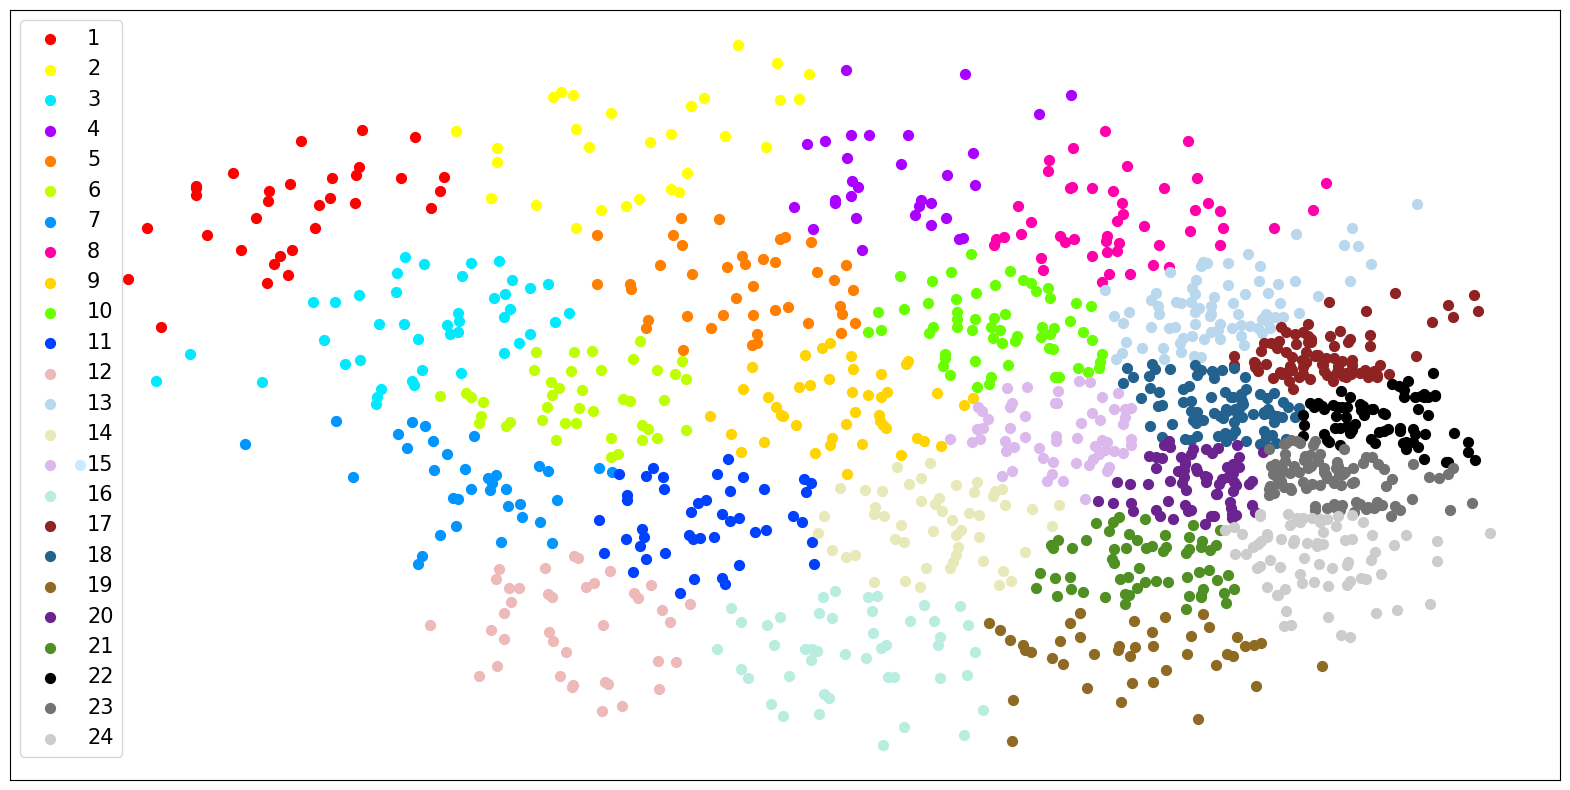
\includegraphics[scale=0.22]{fuzzycmeans_k24_noweights.png}
        \label{fig9}}

    \caption{K-Means, GMM, Agglomerative and Fuzzy C-Means for 24 clusters with 9 indicators.}
        
\end{figure}


\begin{table}[ht]
    \begin{center}
        \caption{Rand Index for 24 clusters}
        \renewcommand{\arraystretch}{1.25}
        \begin{tabular}{ |c|c|c|c|c|c| } 
            \hline
            & KM & GMM & Agg & Fuzzy & QS \\
            \hline
            KM & 1 &  &  &  &  \\
            \hline
            GMM & 0.879644 & 1 &  &  & \\ 
            \hline
            Agg & 0.940349 & 0.880343 & 1 &  & \\ 
            \hline
            Fuzzy & 0.896166 & 0.842625 & 0.885155 & 1 & \\
            \hline
            QS & 0.916113 & 0.872567 & 0.913869 & 0.866017 & 1 \\
            \hline
        \end{tabular}
    \end{center}
\end{table}

\begin{table}[ht]
    \begin{center}
        \caption{Cluster Sizes for 7 clusters}
        \renewcommand{\arraystretch}{1.0}
        \begin{tabular}{ |c|c|c|c|c| } 
            \hline
            & KM & GMM & Agg & Fuzzy \\
            \hline
            1 & 29 & 29 & 30 & 32\\
            \hline
            2 & 24 & 23 & 18 & 29\\ 
            \hline
            3 & 32 & 6 & 43 & 43\\ 
            \hline
            4 & 15 & 29 & 35 & 31\\
            \hline
            5 & 30 & 20 & 33 & 41\\
            \hline
            6 & 41 & 34 & 31 & 42\\
            \hline
            7 & 24 & 52 & 40 & 36\\
            \hline
            8 & 41 & 33 & 26 & 48\\
            \hline
            9 & 30 & 45 & 18 & 44\\ 
            \hline
            10 & 38 & 37 & 44 & 60\\ 
            \hline
            11 & 45 & 44 & 57 & 45\\
            \hline
            12 & 71 & 55 & 49 & 39\\
            \hline
            13 & 47 & 31 & 77 & 79\\
            \hline
            14 & 38 & 65 & 67 & 52\\
            \hline
            15 & 81 & 37 & 40 & 59\\
            \hline
            16 & 60 & 72 & 42 & 46\\ 
            \hline
            17 & 48 & 32 & 111 & 86\\ 
            \hline
            18 & 90 & 60 & 49 & 83\\
            \hline
            19 & 107 & 62 & 80 & 42\\
            \hline
            20 & 87 & 121 & 77 & 67\\
            \hline
            21 & 59 & 127 & 29 & 61\\
            \hline
            22 & 44 & 129 & 132 & 74\\
            \hline
            23 & 129 & 84 & 69 & 92\\
            \hline
            24 & 98 & 81 & 111 & 77\\
            \hline
        \end{tabular}
    \end{center}
\end{table}


\section{Conclusion}








\section*{Acknowledgment}

The preferred spelling of the word ``acknowledgment'' in America is without 
an ``e'' after the ``g''. Avoid the stilted expression ``one of us (R. B. 
G.) thanks $\ldots$''. Instead, try ``R. B. G. thanks$\ldots$''. Put sponsor 
acknowledgments in the unnumbered footnote on the first page. \\


\begin{thebibliography}{00}
\bibitem{b1} Ackermann, M. R., Blömer, J., Kuntze, D., \& Sohler, C. 2014. Analysis of agglomerative clustering. Algorithmica, 69, 184-215.
\bibitem{b2} Savaresi, S. M., Boley, D. L., Bittanti, S., \& Gazzaniga, G. (2002, April). Cluster selection in divisive clustering algorithms. In Proceedings of the 2002 SIAM International Conference on Data Mining (pp. 299-314). Society for Industrial and Applied Mathematics.
\bibitem{b3} Likas, A., Vlassis, N., \& Verbeek, J. J. (2003). The global k-means clustering algorithm. Pattern recognition, 36(2), 451-461.
\bibitem{b4} Bezdek, J. C., Ehrlich, R., \& Full, W. (1984). FCM: The fuzzy c-means clustering algorithm. Computers \& geosciences, 10(2-3), 191-203.
\bibitem{b5} Khan, K., Rehman, S. U., Aziz, K., Fong, S., \& Sarasvady, S. (2014, February). DBSCAN: Past, present and future. In The fifth international conference on the applications of digital information and web technologies (ICADIWT 2014) (pp. 232-238). IEEE.
\bibitem{b6} Wang, Z., Da Cunha, C., Ritou, M., \& Furet, B. (2019). Comparison of K-means and GMM methods for contextual clustering in HSM. Procedia Manufacturing, 28, 154-159.
\bibitem{b7} Elbawab, R. (2022). University Rankings and Goals: A Cluster Analysis. Economies, 10(9), 209.
\bibitem{b8} Stoupas, G., Sidiropoulos, A., Katsaros, D., \& Manolopoulos, Y. (2021). Ranking universities via clustering. In Proceedings of the 18th International Conference on Scientometrics \& Informetrics (ISSI), Leuven, Belgium.
\bibitem{b9} Stoupas, G., Sidiropoulos, A., Katsaros, D., \& Manolopoulos, Y. (2021). When universities rise (Rank) high into the skyline. COLLNET Journal of Scientometrics and Information Management, 15(2), 241-258.
\bibitem{b10} Stoupas, G., Sidiropoulos, A., Gogoglou, A., Katsaros, D., \& Manolopoulos, Y. (2018). Rainbow ranking: an adaptable, multidimensional ranking method for publication sets. Scientometrics, 116(1), 147-160.
\bibitem{b11} Saisana, M., \& d’Hombres, B. (2008). Higher education rankings: Robustness issues and critical assessment. How much confidence can we have in Higher Education Rankings.
\bibitem{b12} Hu, S. (2007). Akaike information criterion. Center for Research in Scientific Computation, 93, 42.
\bibitem{b13} Neath, A. A., \& Cavanaugh, J. E. (2012). The Bayesian information criterion: background, derivation, and applications. Wiley Interdisciplinary Reviews: Computational Statistics, 4(2), 199-203.
\bibitem{b14} Wickelmaier, F. (2003). An introduction to MDS. Sound Quality Research Unit, Aalborg University, Denmark, 46(5), 1-26.
\bibitem{b15} Do, C. B., \& Batzoglou, S. (2008). What is the expectation maximization algorithm?. Nature biotechnology, 26(8), 897-899.

\end{thebibliography}
\vspace{12pt}

\end{document}

